\chapter{Project Selection and Needs Identification}
\label{chapter:projectSelection}
\graphicspath{ {./chapter02/Fig} }

\begin{itquote}
For every problem there is a solution that is simple, neat, and
wrong.---H.L. Mencken
\end{itquote}

Traditionally, companies have organized resources based on functions
such as accounting, engineering, finance, manufacturing, and marketing.
It is often more effective to organize around projects that are of
significant value and align resources to meet the needs of the project.
This means that traditional departments and middle management are being
de-emphasized and the role of projects is growing. Capstone design
projects provide a great opportunity to gain experience in the
management and execution of a project. One of the first and most
important decisions encountered is selecting a project to pursue.

The objective of this chapter is to provide pragmatic guidance in the
project selection phase. A description of design and engineering
projects is presented, followed by advice on how projects can be
selected by engineering students who wish to put design principles into
practice. The chapter addresses how to identify the needs of the
end-user and provides guidance for conducting background research. All
of this information is brought together in a Problem Statement that
identifies the needs, the goals of the project, and research on the
technology.

\section*{Learning Objectives}
\noindent\rule{\linewidth}{1pt}
By the end of this chapter, the reader should:
\begin{itemize}
\item
  Have an understanding of the types of projects that electrical and
  computer engineers undertake.
\item
  Understand and be able to apply criteria for project selection.
\item
  Know how to determine, document, and rank end-user needs.
\item
  Be aware of resources available for conducting research surveys.
\item
  Have selected a project concept and developed a Problem Statement.
\end{itemize}

\section{Engineering Design Projects}
\label{section:engineering-design-projects}

This section provides a classification of design and describes some of
the types of projects undertaken by practicing engineers and those
tackled in student projects. In reality, most projects don't fit neatly
into the categories presented, but are some combination of them. The
objective of a design project is to create a new
\emph{\textbf{artifact}} (system, component, or process) to meet a given
need. Within the design domain there are different types of designs that
are classified broadly into three categories of Creative, Routine, and
Variant designs {[}Cro00{]}.

\emph{\textbf{Creative designs}} represent new and innovative products.
An example of a creative design is the Palm Pilot Personal Digital
Assistant (PDA). While the idea for the PDA had been around for awhile,
earlier attempts at developing the technology, notably the Apple Newton,
were unsuccessful. This was primarily due to unreliable handwriting
recognition that frustrated the user. However, Palm Computing had the
creative idea to develop a simplified handwriting language, Graffiti,
which eliminated the need for natural handwriting recognition. The Palm
Pilot is a great example of a creative design---it is simple (four basic
functions), fits in your pocket, and is easy to use. This innovation
spawned a huge hand-held computing industry.

\emph{\textbf{Variant designs}} are variations of existing designs,
where the intent is to improve performance or add features to an
existing system. Many engineering projects fall into this category. For
example, the objective may be to increase accuracy or system throughput.

\emph{\textbf{Routine designs}} represent the design of devices for
which theory and practice are well-developed. Examples are DC power
supplies, analog and digital filters, and basic digital components such
as adders and comparators. Routine designs are often components of more
complex creative and variant designs.

Within these three categories of design, there are many different types
of projects. \emph{Systems engineering and systems integration projects}
represent the synthesis of many subsystems into a larger system. They
may be creative or variant designs, but have unique challenges since
they are typically large and involve many people and technologies.
Adherence to good design processes is important for their success.
Engineers are often engaged in \emph{systems test}, where the objective
is to ensure that a system meets stated requirements and the needs of
the user. Examples include the testing of systems for use in space and
military environments.

The objective in \emph{experimental design} \emph{projects} is to design
experimental procedures and apparatus for determining the
characteristics of a system. For example, an engineering team may test a
system under a variety of operating conditions. 
Example~\ref{example:aerialSurveillanceNeeds} presented
later in the chapter is such a project, where the objective was to
design a series of experiments to test the feasibility of gigabit
Ethernet technology in a military environment. The test explored the
impact of environmental factors such as temperature and vibration, and
further used this data to estimate the operating lifetime of the
Ethernet board. Upon completion of this project, the team made
recommendations as to the allowable operating ranges of the technology.

The objective in \emph{analysis projects} is to analyze some aspect of
an existing system to improve or correct it. For example, a system or
process may be failing in the field and the source of the failure
unknown. Tools such as the Failure Mode Effects and Analysis technique
may be applied in this situation to identify the sources of failure. In
t\emph{echnology evaluation} \emph{projects}, technologies are assessed
to determine if they can be used in a given application. This may be to
determine if the technology can improve an existing system, or to
characterize its operating performance.

The objective of a \emph{research project} is to perform research or
experiments with the goal of discovering or creating a new technology.
The fundamental difference between this and other types of projects is
that the ultimate outcomes are unknown. Most engineering research falls
under the category of \emph{applied research}. This refers to the
creation of new technology or systems based on existing technology and
theory developed from fundamental research. \emph{Fundamental research}
emphasizes the discovery of new scientific principles without
necessarily having an intended application. Fundamental research is very
valuable, but not typically a part of design projects.

\section{Sources of Project Ideas}
\label{section:sources-of-project-ideas}

Depending upon your situation, you may have the opportunity to identify
and select your project. The list below provides some places to search
for project ideas:

\begin{itemize}
\item
  \emph{Industry sponsored projects.} Many companies will sponsor
  projects and are happy to do so, particularly if you have worked for
  them on an internship.
\item
  \emph{Engineers without Borders
  (\href{http://www.ewb-usa.org}{www.ewb-usa.org})}. This organization
  sponsors student projects to improve the quality of life in developing
  countries.
\item
  \href{http://www.FreeRandD.com}{\emph{www.FreeRandD.com}}. This is a
  clearinghouse for businesses and students teams to collaborate on
  projects. It allows businesses to post capstone project ideas for
  students to work on, while students can post resumes and project
  interests.
\item
  \emph{Your campus and local community.} In our school, a number of
  student teams have identified novel projects by asking other
  departments on campus for ideas. They have also been successful in
  approaching local community organizations for ideas, such as museums
  and research institutes.
\item
  \emph{Brainstorm.} Get together with a group of your peers and
  brainstorm on project ideas. You will be surprised at how many project
  ideas you can develop in a good brainstorming session (see Chapter~\ref{chapter:conceptGen}).
  Do not only consider project ideas, but also brainstorm to identify
  problems that need solutions.
\end{itemize}

\section{Project Feasibility and Selection Criteria}
\label{section:project-feasibility-and-selection-criteria}
This section provides questions to consider when examining the
feasibility of a project. George H. Heilmeier (an electrical engineer
who has held positions as Chief Technology Officer of Texas Instruments,
Director of the Defense Advanced Research Projects Agency, and CEO of
Bellcore) developed a set of questions to answer when starting a new
project {[}Sha94{]}. Heilmeier argued that all projects must be tied to
the goals of the organization, and applied this by asking the following
questions:

\begin{itemize}
\item
  What are you trying to do? Articulate your goals using absolutely no
  jargon.
\item
  How is it done today, and what are the limitations of current
  practice?
\item
  What is new in your approach, and why do you think it will be
  successful?
\item
  Who cares? If you are successful, what difference will it make?
\item
  What are the risks and payoffs?
\item
  How much will it cost? How long will it take?
\item
  What are the midterm and final exams to check for success?
\end{itemize}

Heilmeier credits successful completion of projects that he managed to
answering these questions up-front and adhering to disciplined project
management processes.

A second perspective is offered from an organizational project
management viewpoint {[}Gra02{]} that provides the following criteria
for project selection:

\begin{itemize}
\item
  \emph{The project must be tied to the mission and vision of the
  organization.} Believe it or not, organizations often spend resources
  fruitlessly on projects that don't meet this criterion. To be fair,
  there is always risk associated with a project and it is sometimes
  hard to judge exactly how well a project meets this criterion. For
  engineers who are new to an organization, it is hard to judge a
  project's importance relative to the mission and goals, but if you
  find yourself in this situation, do not be afraid to ask some
  questions. Novices ask basic questions that are often overlooked by
  those who are highly experienced or intimately involved in a project.
\item
  \emph{Must have payback.} An economic analysis should be done to
  estimate if the project will make a profit. Much of this is outside
  the scope of this text, requiring marketing and financial analyses.
  Chapter~\ref{chapter:projectManagement} covers the basics of project cost estimation that will help
  in trying to answer this question.
\item
  \emph{Should have selection criteria.} Sound criteria for selecting
  among competing projects should be employed. The example at the end of
  this section demonstrates the application of criteria in project
  selection.
\end{itemize}

\begin{itemize}
\item
  \emph{Objectives of the Project should be SMART: Specific, Measurable,
  Assignable, Realistic, Time-Related}. Chapter~\ref{chapter:requirementSpec} addresses how to
  determine project requirements that are Specific and Measurable.
  Assignable, Realistic, and Time-Related all refer to project
  management aspects that are covered in Chapter~\ref{chapter:projectManagement}. The objective is to
  develop tasks that are assigned to groups or individuals and
  realistically can be completed in the given timeframe.
\end{itemize}

Example~\ref{example:projectSelectionModel} demonstrates how to apply a project selection
model using a method known as the Analytical Hierarchy Process. AHP is a
decision making method that is described in Appendix~\ref{appendix:DecisionMakingAHP}
 and is utilized frequently throughout the text -- \textbf{the reader should read 
 Appendix~\ref{appendix:DecisionMakingAHP} prior to proceeding with this example}.

\begin{example}{ A project selection model for capstone design.}
\label{example:projectSelectionModel}

Assume that you are part of a capstone design team that has the
opportunity to select their project from competing project ideas. The
steps in making a decision using AHP are to select the criteria that
drive the decision, determine relative weights of the criteria, rate the
alternatives (in this case project concepts) against the criteria, to
compute a weighted score for each of the alternatives, and then review
the decision.

\ul{Step 1: Determine the selection criteria}

To select the criteria, assume that the team brainstorms to determine
the following criteria that interest the team members:

\begin{quote}
A -- Match to team skills
B -- Technical complexity
C -- Creativity
D -- Market potential
E -- Industry sponsorship
\end{quote}

\ul{Step 2: Determine the criteria weightings}

Assume the team applies the method of pairwise comparison to determine
the weights as shown in Appendix~\ref{appendix:DecisionMakingAHP}. 
In order to do so, the team
systematically compares each criterion to all others using the following
scale of relative importance:

1 = equal, 3 = moderate, 5 = strong, 7 = very strong, 9 = extreme.

Again, details of pairwise comparison are outlined in 
Appendix~\ref{appendix:DecisionMakingAHP} and the
results are below. \\


\begin{tabular}{ |> {\columncolor{Gray}} c  |c|c|c|c|c|c|} 
\hline
\rowcolor{Gray}
Criteria & A & B & C & D & E & Weight \\ 
\hline
A & 1 & 5 & 5 & 3 & 3 & 0.52 \\
\hline
B & 1/5 & 1 & 3 & 1/3 & 1/3 & 0.12 \\
\hline
C & 1/5 & 1/3 & 1 & 1 & 3 & 0.09 \\
\hline
D & 1/3 & 3 & 1 & 1 & 5 & 0.18 \\
\hline
E & 1/3 & 3 & 1/3 & 1/5 & 1 & 0.09 \\
\hline
\end{tabular}
\\

This is an important step and one often overlooked -- the team has
identified what is important to it in project selection. It is clear
that match to the team skills (criterion A) is most important, by a
large margin, followed by market potential.

\ul{Step 3: Identify and rate alternatives relative to the criteria}

Assume that the team identifies three potential projects ideas: 1 --
IEEE sponsored robot competition, 2 -- Industry sponsored project to
design a new test protocol, and 3 -- Design of an item-finder device to
help people locate lost items. Furthermore, the team goes through the
process of rating each project relative to the criteria as outlined in
Appendix~\ref{appendix:DecisionMakingAHP}. 
These ratings are reflected in the decision matrix in the
next step.

\ul{Step 4: Compute scores for the alternatives}

The decision matrix below is constructed and the scores for the
alternatives determined.


\begin{tabular}{|l|c|c|c|c|}
\hline
\rowcolor{Gray}
 & & \multicolumn{3} {c|} {Alternatives} \\ \hhline{|~|~|-|-|-|}
\rowcolor{Gray}
 \multirow{-2}{*}{Selection Criteria} & \multirow{-2}{*}{Weights}  & Project 1 & Project 2 & Project 3 \\ \hline
A (Match to skills) & 0.52 & 0.40 & 0.20 & 0.40 \\  \hline
B (Technical Complexity) & 0.12 & 0.40 & 0.30 & 0.30 \\ \hline
C (Creativity) & 0.09 & 0.45 & 0.20 & 0.35 \\ \hline
D (Market potential) & 0.18 & 0.05 & 0.35 & 0.60 \\ \hline
E (Industry sponsorship) & 0.09 & 0.00 & 1.0 & 0.00 \\ \hline
Score & & 0.31 & 0.31 & 0.38 \\ \hline
\end{tabular}\\


\ul{Step 5: Review the decision}

Project 3 (item finder) is rated the highest among the three choices
based upon the weights determined by the team members. It is a good
match to the team skills, but also matches their desire to solve a
problem with good market potential. The remaining two projects are rated
about equal.

\end{example}

\section{Needs Identification}
\label{section:needs-identification}

Often a customer, client, or supervisor comes to you with a problem to
solve and you must determine the needs or requirements for the solution
to the problem. In other words, determine the \emph{voice of the
customer}. This seems like a simple statement---ask the customer what
they want and you are done, right?

As an illustration, let's say a client comes to you with the following
request---\emph{The traffic at the front of campus is too congested. I
would like you to design a new traffic lane for northbound traffic
exiting at the intersection at the front of the college.} So you design
this new lane and have it added to the intersection. However, you find
out three months later that the traffic congestion has decreased a
little bit, but it is still a significant problem. So what went wrong?
Clearly you did what was asked of you, but the problem was not solved,
meaning that you were solving the wrong problem. The real problem was to
improve the flow of traffic at the entrance. In this case, the client
gave both the problem and the solution all in one statement. That is
fine if a careful feasibility study was done and it was known that the
additional traffic lane would alleviate the problem, but that was not
the case here. This hypothetical situation is not so far fetched and
happens in practice via neglect to do the up-front research or because
underlying assumptions change. The point is that the \ul{correct}
problem should be identified and solved.

It would be better if the client had simply asked to improve the traffic
flow, providing the opportunity to analyze the situation and develop
different design options. Some questions to be asked in this situation
are: \emph{How much additional traffic is there? At what times does this
happen? Where is the traffic coming from? What is an acceptable waiting
time at the intersection?} It may be that several new lanes are needed,
or perhaps the sequencing of the traffic signals is wrong, or maybe a
new entrance could be added for less cost and improved traffic flow.

The lesson is that customers often come with the problems and solution
all wrapped up together. When this is done, the \emph{\textbf{design
space}}, the space of all possible solutions to the problem, is
unnecessarily limited. Be ready to tactfully challenge the assumptions
and ask questions to get to the root of the problem. Ask clarifying
questions, analyze, pick apart the request, and focus on the problem,
not the solution.

Researchers and practitioners have examined the problem of eliciting
needs, and it is an important pre-requisite for developing good
engineering requirements specifications. Ulrich and Eppinger {[}Ulr03{]}
proposed a process for obtaining the \emph{voice of the customer} using
the following five steps: 1) Gather raw data from users; 2) Interpret
raw data in terms of needs; 3) Organize needs into a hierarchy; 4)
Determine the relative importance of the needs; and 5) Review the
outcomes and the process. Each of these steps is described in the
following sections.

\subsection*{ Step 1: Gather Raw Data from Users}

\textbf{DILBERT\textsuperscript{®} by Scott Adams}

\begin{figure}[h]
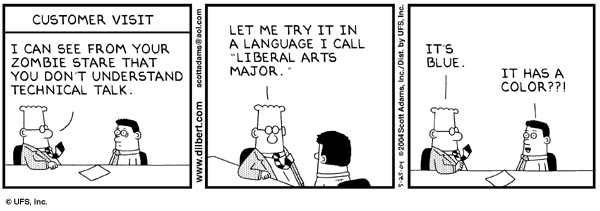
\includegraphics[width=5.5in,height=1.9in]{image1.png}
\caption{ The difficulties of communicating with the customer. (Dilbert © United Feature Syndicate. Reprinted by
permission.)}
\label{figure:dilbertCommunication}
\end{figure}


This is often accomplished via interviews with supervisors, key users,
or people from the client organization. In cases where new products are
being developed, focus groups are often employed. The advantage of
interviews and focus groups is that they provide the opportunity for
dialogue with the user where new ideas, concepts, and needs may emerge.
Another option is direct observation, where the team goes out and
examines the system in use and develops concepts for improving it. IDEO
Corporation is an innovative and successful company that designs new
products and systems. They rely heavily on direct observation as a
technique for successfully developing innovative products {[}Kel01{]}.
For example, IDEO was asked by a client to develop a new medical
instrument for balloon angioplasty used in hospital operating rooms. A
critical requirement from the user was that only one hand could be used
to operate the device because the technician's other hand had to be free
during the procedure. From direct observation, the IDEO design team
found that even though the current system was designed for one-hand use,
it was impractical, and the technicians actually used both hands. IDEO
designed and developed a two-handed pump that not only worked better
than the one handed pump, but was quieter, easier to read, and had
increased precision. This is another example of the customer specifying
the solution as part of the problem statement.

Ulrich and Eppinger provide the following questions to ask during an
interview:

\begin{itemize}
\item
  When and why do you use this type of product (system)?
\item
  Walk us through a typical session using the product.
\item
  What do you like about the existing products?
\item
  What do you dislike about the existing products?
\item
  What issues do you consider when purchasing the product?
\item
  What improvements would you make to the product?
\end{itemize}

\subsection*{Step 2: Interpret the Raw Data in Terms of Needs}


In this step the raw data is translated into customer needs. The needs
are expressed in terms of what the system must do (a requirement) as
opposed to how it is done. Statements of the customer's needs are known
as \textbf{\emph{marketing requirements}} or \emph{\textbf{marketing
specifications}}. For example, ``\emph{The system should have
high-quality audio}'' is a need or marketing requirement from the
customer regarding performance, but says nothing about how it will be
achieved. Marketing requirements are short sentences that describe the
need in the language of the customer. They typically do not have a
numerical target and are described as a state of being for the system.
Other examples of marketing requirements are, ``\emph{The system should
be easy-to-use,}'' and ``\emph{The system should be able survive a drop
from the runner's height.}''

\subsection*{Step 3: Organize Needs into a Hierarchy}

The marketing requirements are organized into a hierarchy of needs
arranged from the most general to the most specific in successive levels
of detail as required by the problem. It is organized by functional
similarity, not as hierarchy of importance (that is the next step). This
hierarchy is referred to as an \emph{\textbf{objective tree}}. An
example objective tree for a portable audio device intended for use by
runners is shown in Figure~\ref{figure:audioPortable}. The three high-level objectives
determined were high-quality audio, portable, and easy-to-use. Each of
these is further sub-divided into the characteristics that support the
higher level. For example, portability is divided into the needs of
lightweight, small, ergonomic, and the ability to operate in the
environment. The environmental need is further expanded into needs that
support it.

\begin{figure}[h]
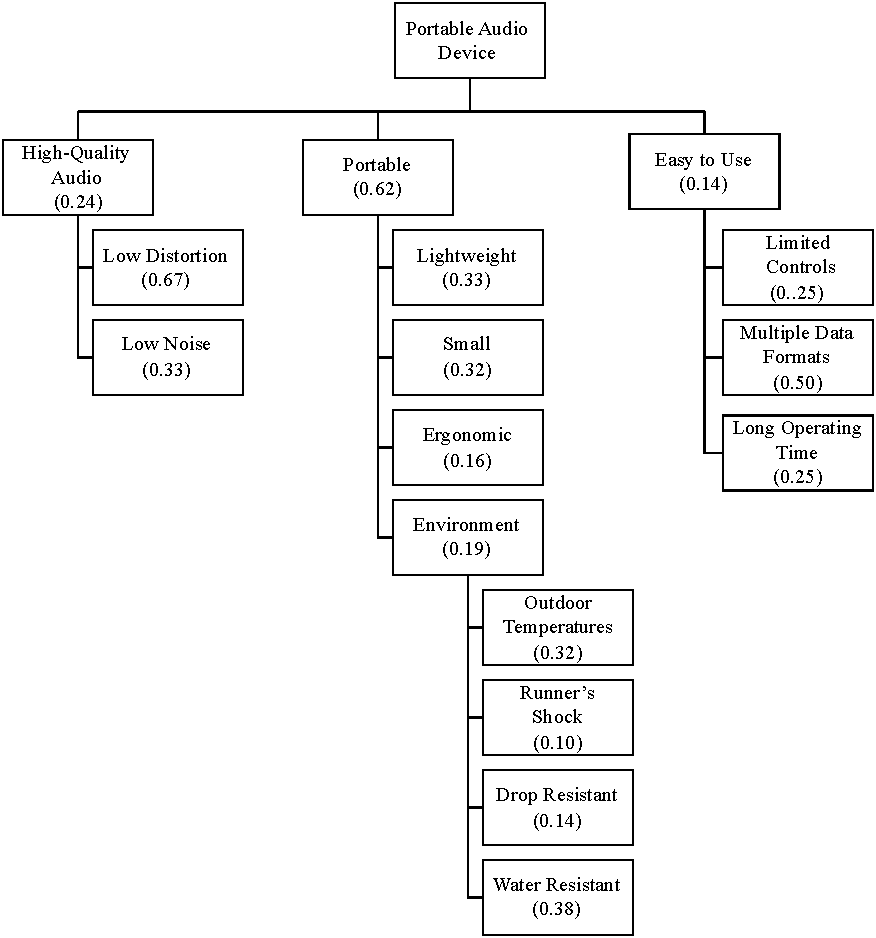
\includegraphics[width=5.2in,height=5.6in]{image2}
\caption{Objective tree for a portable audio device to be
used by runners. The weights reflect the relative importance of needs at
each level in the hierarchy as determined in Step 4 of the
process.}
\label{figure:audioPortable}
\end{figure}

\subsection*{Step 4: Determine the Relative Importance of the Needs}


The relative importance of the needs is determined based upon the user
needs. As we saw in Example~\ref{example:projectSelectionModel} and as presented in 
Appendix~\ref{appendix:DecisionMakingAHP}, the
pairwise comparison is a good technique for determining relative
importance and weighting of needs. In pairwise comparison, all needs are
systematically compared to all other needs at the same level in the
hierarchy. An example pairwise comparison table for this problem is
shown in Table~\ref{table:highQualityAudio} 
with the resulting weights for each need indicated.
This shows that portability is the most important need, followed by
audio quality and ease-of-use. The weights are also reflected in the
objective tree in Figure~\ref{figure:audioPortable}. In addition, the needs at each sublevel in
the hierarchy are compared, the results of which are reflected in 
Figure~\ref{figure:audioPortable}. The rankings are used in later chapters to compare design
alternatives.

\begin{table}[h]
\centering
\begin{tabular} {|> {\columncolor{Gray}} l|c|c|c||c|}
\hline
\rowcolor{Gray}
                             & High-Quality Audio & Portable & Easy-to-Use & Weight \\
\hline
High-Quality Audio & 1 & 1/3 & 2 & 0.24 \\
\hline
Portable & 3 & 1 & 4 & 0.62 \\
\hline
Easy-to-Use & 1/2 & 1/4 & 1 & 0.14 \\
\hline
\end{tabular}
\caption{Pairwise comparison matrix for ranking the
highest-level needs of the portable audio device. This comparison should
be carried out for all levels of the objective tree.}
\label{table:highQualityAudio}
\end{table}


\subsection*{Step 5: Review the Outcomes and the Process}

The design process and all of its sub-processes are methods for making
good decisions, and this technique for needs identification is no
different. There is a certain amount of subjectivity and judgment that
goes into it; the end result should be reviewed to determine if it makes
sense. The objective is to challenge assumptions, fully identify the
problem, and make informed decisions.

The three outcomes of this process are the marketing requirements that
identify the needs, an objective tree that provides a hierarchical
representation of the needs, and a ranking of the relative importance of
needs. This process may seem as though it does not apply to student
design projects, but in reality it does. The questions in this chapter
are certainly candidates to ask when working on company-sponsored
projects. If it is not a company sponsored project, the user needs
should still be considered. For example, questions can be asked of
friends and co-workers who are potential users of the system, focus
groups can be formed, surveys administered, and Internet bulletin boards
and discussion groups employed to gather this information.

\section{The Research Survey}
\label{section:the-research-survey}

It is important to conduct a thorough research survey while defining the
project concept. Failure to do so may translate into time and money
spent reinventing the wheel, while not taking full advantage of existing
components, knowledge, practices, and technology. During the research
phase, competing systems and technologies are identified, and based upon
them the project concept refined, or in some cases abandoned. The
character and strategy of the research survey is driven by the nature of
the project. In general, the objective is to develop an understanding of
the underlying scientific principles and demonstrate a familiarity with
the state-of-the-art in the particular field. Some questions to be
answered in the research survey are:

\begin{itemize}
\item
  What is the basic theory behind the concept?
\item
  How is it currently being done?
\item
  What are the limitations of current designs or technology?
\item
  What are the similarities and differences between your concept and
  existing technologies?
\item
  Are there existing or patented technologies that may be relevant to
  the design? If so, what are they and why are they relevant?
\end{itemize}

\textbf{Internet Searching}

The Internet is a powerful, fast, and readily accessible source for
conducting research. There are many excellent search engines for
locating web resources, but understand that it is important to go beyond
the well-known search engines and beyond the Internet in the survey.

One of the risks, and also one of the wonderful things, about the
Internet is that virtually anybody can post information. It is important
to analyze websites to ensure that they are reliable and credible. There
are resources available that provide pointers on how to evaluate this
credibility {[}Mci02, Sch98{]}, and a little common sense goes a long
way. One of the important things to look for is authorship---the author
should be clearly identified and any affiliations listed. Carefully
determine whether the information is subjective opinion or possibly a
commercial for a product. Credible sites should provide references to
original sources of material. Another step is to verify website content
in print media or other reliable sources.

There are thousands of search engines available, making the task of
selecting one challenging. Also, there are different types of search
engines: text (search for the text or keywords; subject heading or
full-page text search), indexed (information categorized into
directories), meta-search (engines that search other engines), and
natural language processing (allowing natural language queries). A
listing of search engines to try are
\href{http://www.altavista.com}{www.altavista.com},
\href{http://www.AskJeeves.com}{www.AskJeeves.com},
\href{http://www.google.com}{www.google.com},
\href{http://www.kartoo.com}{www.kartoo.com}, and
\href{http://www.yahoo.com}{www.yahoo.com}. The Librarian's Index to the
Internet, \href{http://www.lii.org}{www.lii.org} is a collection
selected and evaluated by librarians, and according to their website, it
is \emph{a} ``\emph{well-organized point of access for reliable,
trustworthy, librarian-selected Internet resources}.'' This information
may change rapidly and represents current information at the time of
publication.

\textbf{Electrical and Computer Engineering Resources}

Realize that the major search engines will not find all information
available on the Internet. There are many websites with specialized
search capabilities related to electrical and computer engineering
design.

\begin{itemize}
\item
  EE Product Center,
  \href{http://www.EEProductCenter.com}{www.EEProductCenter.com}. A
  website for locating electronic components and their manufacturers. It
  provides links to product datasheets and application notes. It has a
  keyword search engine and a tree structure search for finding
  components. For example, you can start with Op Amps and delve into
  sub-categories such as Precision and High-Speed.
\item
  Circuit Cellar,
  \href{http://www.CircuitCellar.com}{www.CircuitCellar.com}. This
  companion website for the magazine is a great reference for designers.
  It emphasizes embedded systems and electronics projects with many
  tutorial articles and project ideas.
\item
  Datasheet Catalog,
  \href{http://www.DatasheetCatalog.com}{www.DatasheetCatalog.com}. A
  datasheet source for electronic components and semiconductors.
\item
  Dr. Dobbs, \href{http://www.ddj.com}{www.ddj.com}. The magazine and
  companion website are a resource for software developers that includes
  tips and tutorials.
\item
  EE Times, \href{http://www.EETimes.com}{www.EETimes.com}. Industry
  newspaper for electrical engineering field with information on current
  technology developments.
\item
  Electronic Design Magazine,
  \href{http://www.EDNmag.com}{www.EDNmag.com}. This is free magazine
  for electrical design engineers that provides information on the
  latest products. The website has a number of categorized technical
  resources and a design ideas section.
\item
  ON Semiconductor, \href{http://www.OnSemi.com}{www.OnSemi.com}. ON
  Semiconductor is a supplier of semiconductors for a wide range of
  applications, with a particular emphasis on power management. The
  website has a searchable database of over 15,000 components, and
  provides guidelines for component selection based on different
  applications.
\item
  The Thomas Register,
  \href{http://www.ThomasRegister.com}{www.ThomasRegister.com}. This is
  a source for finding companies and products in North America. It
  allows searches for parts and equipment that may be used in a design
  project. It provides profiles of companies that meet the search
  criteria and describes the products they make.

  In addition, most manufacturers of electronic components have websites
  providing product datasheets and application notes for their products.
  Application notes demonstrate how to use components in real
  applications. Examples are Dallas Semiconductor, Fairchild
  Semiconductor, Motorola, and Texas Instruments.
\end{itemize}

\textbf{Government Resources}

\begin{itemize}
\item
  US Bureau of Labor Statistics, \url{http://stats.bls.gov}. This has
  valuable information on consumer spending information, allowing one to
  determine things such as how much people spend and what they spend it
  on. It also profiles specific industries and forecasts employment in
  different industry sectors.
\item
  US Government Official WebPortal,
  \href{http://www.FirstGov.gov}{www.FirstGov.gov}. This is an entrance
  to all US government web resources.
\item
  US Patent Office, \href{http://www.uspto.gov}{www.uspto.gov}. A
  searchable database of all patents back to 1790. Full text searches
  are available back to 1976 and full images back to 1790. It has
  information on the basics of patents, trademarks, and copyrights.
\end{itemize}

\textbf{Journal and Conference Papers}

The search should include journal and conference papers if technically
detailed information on the latest theory or applications is needed.

\begin{itemize}
\item
  ACM (Association for Computing Machinery) Digital Library,
  \href{http://www.acm.org}{www.acm.org}. Provides abstracts (full text
  for subscribers) for ACM journals and conference proceedings.
\item
  Compendex,
  \href{http://www.engineeringvillage2.org}{www.engineeringvillage2.org}.
  This provides indices to journal and conference papers in a broad
  scope of engineering fields, referencing material back to 1970.
\item
  IEEE (Institute of Electrical and Electronics Engineers) Xplore
  Electronic Library, \href{http://www.ieee.org}{www.ieee.org}. Provides
  abstracts (full text for subscribers) to all IEEE journals,
  transactions, magazines, and conference subscriptions published since
  1988. Abstracts for all IEEE standards are publicly available.
\end{itemize}

\section{Needs and Objectives Statements}
\label{section:needs-and-objectives-statements}

Two parts of the Problem Statement are the needs and objectives
statements. The \emph{needs statement} identifies and motivates the need
for the project and should:

\begin{itemize}
\item
  Briefly and clearly state the need being addressed.
\item
  Not provide a solution to the problem.
\item
  Provide supporting information collected as outlined in Section~\ref{section:needs-identification}.
\item
  Provide any supporting statistics and anecdotes that support the need.
\item
  Describe current limitations.
\item
  Describe supporting processes that are needed to understand the need.
  This is particularly important in industry-sponsored projects having
  specific needs that may not be clear to the average person.
\end{itemize}

The \emph{objectives statement} typically ranges from one or two
sentences to one or two paragraphs in and should:

\begin{itemize}
\item
  Summarize what is being proposed to meet the need.
\item
  Provide some preliminary design objectives (detailed requirements are
  developed later).
\item
  Provide a preliminary description of the technical solution, avoiding
  a detailed description of the implementation. Often the input and
  output behavior of the system are described. The complete solution is
  not usually posed until after the engineering requirements are fully
  determined.
\end{itemize}

Example needs and objectives statements are provided in Examples
\ref{example:iPodNeeds}, \ref{example:intelProNeeds}, and \ref{example:aerialSurveillanceNeeds}.

\begin{example}{iPod Hands-Free Device Needs and Objectives.
\emph{Abstracted from the iPod Hands-Free Device Design Report by
Al-Busaidi, Bellavia, and Roseborough {[}Alb06{]}. }}
\label{example:iPodNeeds}
\ul{Need:} According to AppleInsider, approximately 10.3 million people
owned iPods at the end of 2004 and many of the owners used them while
operating their automobiles. The National Highway Traffic Safety
Administration estimates that driver distraction is a contributing cause
of 20 to 30 percent of all motor vehicle crashes -- or 1.2 million
accidents per year. One research study has estimated that driver
inattention may cause as many as 10,000 deaths each year and
approximately \$40 billion in damages. iPods can present a distraction
to drivers that is similar to cell phones in that the driver's attention
is divided between controlling the steering wheel, watching the road,
and navigating controls on the iPod. A system is needed to allow users
to navigate among the music selections of their iPod without distracting
their attention from the road.

\ul{Objective:} The objective of this project is to design and prototype
a device that will make the iPod safer to use while driving an
automobile, by allowing hands-free control of the iPod. The device will
interact with the user using spoken English commands. The user will be
able to issue simple voice commands to the device to control the
operation of the iPod. In turn, the device will communicate information
verbally, such as song titles that are displayed on the iPod screen, to
the user.
\end{example}

\begin{example}{Experimental Design Problem Needs and Objectives.
\emph{Abstracted from the Intel Pro 1000XF Server Testing Design Report
by Esek, Hunt, and Lewis. {[}Ese03{]}. }}
\label{example:intelProNeeds}
\ul{Need:} Our industry sponsor is investigating the performance of
commercial grade gigabit Ethernet fiber optic equipment for computer
data communications in a military environment. The proposed system will
utilize an Intel Pro1000 XF server card. This is a harsh operating
environment and its effects on the performance and lifetime of the
equipment are unknown. The client wishes to understand how the military
environment affects the optical power margin of the Intel Pro 1000 XF
card and associated connectors and cabling.

\ul{Objective:} The goal of this project is to design the experimental
equipment and test procedures to determine the effects of temperature
variations and vibration on the optical power margin and the operating
lifespan of the system.
\end{example}

\begin{example}{Portable Aerial Surveillance Needs and Objectives.
\emph{Abstracted from the PASS Design Report by Andre, Kolb, and Thaler
{[}And06{]}. }}
\label{example:aerialSurveillanceNeeds}
\ul{Need:} Emergencies happen all across the world, all of the time.
There are nearly 2,000,000 reported fires in the United States every
year, and over 90 tactical activations of Pennsylvania's Special
Emergency Response Team which handles barricaded suspects and hostage
situations. There have been over 100 documented riots in the United
States in the past century, with the Los Angeles Riot alone causing \$1
billion in damage. Having an aerial view of these situations would be a
great benefit to the emergency workers on the ground. For example,
police may have to monitor a large crowd or a hostage situation where
aerial surveillance would allow them to observe the situation from a
safe distance and use the footage as evidence in court. Firefighters
could use aerial surveillance to examine fire damaged buildings and
search for victims through the windows of high-rise buildings. In large
cities, emergency organizations often employ helicopters for aerial
surveillance. However, in smaller rural towns, helicopters either take
too long to reach the scene from a nearby city or they are too expensive
to afford. The least expensive two-seat helicopters cost over \$400,000,
while new helicopters cost well over a million dollars with average
operating costs of \$400-\$1000 per hour. There is a need for a low cost
aerial device that can provide emergency workers with overhead
surveillance of emergency situations.

\ul{Objective:} The objective of this project is to design a device that
will provide emergency workers with a live aerial view of a situation at
a cost that small municipalities can afford. The device will deploy
rapidly and record and log video. The camera will also include pan and
zoom functionality to make identification of victims and suspects
easier.
\end{example}

\section{Project Application: The Problem Statement}
\label{section:project-application-the-problem-statement}

A format for a Problem Statement that integrates the elements of this
chapter is as follows:

\begin{itemize}
\item
  \emph{Need.} A statement that identifies the needs of the project.
\item
  \emph{Objective.} Describes the concept proposed to meet the needs
  identified.
\item
  \emph{Background.} A summary of the research survey on the relevant
  technologies and systems. The objective is to provide an introduction
  answer the questions posed in Section~\ref{section:needs-identification}. 
  The length and content of
  this section varies depending upon the project.
\item
  \emph{Marketing Requirements.} Short statements describe the user
  needs.
\item
  \emph{Objective Tree}. A hierarchical representation of the needs
  based on functional similarity with the relative weights of the needs
  identified.
\end{itemize}

\section{Summary and Further Reading}
\label{section:summary-and-further-reading}

This chapter addressed the types of projects that are often undertaken
by engineers and provides guidance in terms of questions to ask when
selecting a project. The success of design projects depends upon
adequately determining the user's needs and desires for the system. A
process developed by Ulrich and Eppinger for needs elicitation was
presented. The three outcomes of this process are: 1) marketing
requirements identifying the customer needs, 2) an objective tree that
hierarchically represents the needs, and 3) a ranking of the relative
importance of the needs. It is important to conduct research on the
concept and related technologies, and pointers for conducting the
research survey were provided. Finally, a format for a Problem Statement
was presented that summarizes the needs, objectives, and research survey
for a design project.

The works by Griffin and Hauser {[}Gri93{]} and Ulrich and Eppinger
{[}Ulr03{]} are readable and more detailed discussions on how to obtain
the voice of the customer. There are also other design books available
that address how to identify needs and develop objective trees
{[}Cro00{]}. Cagan and Vogel {[}Cag02{]} have proposed a process for
product development known as iNPD (integrated new product development)
and provide methods for navigating what they refer to as ``the fuzzy
front end of project definition.''
